\documentclass[a4paper]{article}

%------------------------------------------------------------
\usepackage[a4paper, total={6in, 9in}]{geometry}
\usepackage{amsmath}
\usepackage{booktabs}
\usepackage{caption}
\usepackage{enumitem}
\usepackage{graphicx}
\usepackage{float}
\usepackage{inconsolata}
\usepackage{listings}
\usepackage{pstricks-add}
\usepackage{siunitx}
\usepackage[most]{tcolorbox}
\usepackage{tikz}
\usepackage{epstopdf} %converting to PDF
\usepackage{hyperref}
\usepackage{rotating}

\usetikzlibrary{shapes.geometric}
\usetikzlibrary{calc}

%------------------------------------------------------------
\graphicspath{{./fig/}}

%------------------------------------------------------------
\setlength{\parindent}{0in}

\lstdefinestyle{Python}{
	language        = Python,
	basicstyle      = \ttfamily,
	keywordstyle    = \color{blue},
	keywordstyle    = [2] \color{teal}, % just to check that it works
	stringstyle     = \color{green},
	commentstyle    = \color{red}\ttfamily
}

%------------------------------------------------------------
\newtcblisting[auto counter]{sexylisting}[2][]{sharp corners, 
    fonttitle=\bfseries, colframe=gray, listing only, 
    listing options={basicstyle=\ttfamily,language=Python}, 
    title=Listing \thetcbcounter: #2, #1}

%------------------------------------------------------------
\tikzstyle{block} = [draw, fill=blue!20, rectangle, 
    minimum height=3em, minimum width=3em]
\tikzstyle{sum} = [draw, fill=blue!20, circle, node distance=1cm]
\tikzstyle{input} = [coordinate]
\tikzstyle{output} = [coordinate]
\tikzstyle{pinstyle} = [pin edge={to-,thin,black}]

%------------------------------------------------------------

\begin{document}
\title{SLAM: Map My World}
\author{Shane Reynolds}
\maketitle

\section*{Abstract}

\section{Introduction}
Consider a robot in an unknown environment, with no known map. The robot takes sensor readings and experiences control actions. Based on these observations and actions, the robot must construct a map and localise itself within the map. In robotics, this scenario is known as the \textit{simultaneous localisation and mapping problem}, or SLAM. In simpler terms, using sensor readings and control data, SLAM concurrently constructs an environment map, and determines the robots location and orientation within that map. This is an important problem since odometric data is subject to small perturbations which are introduced from wheel slippage and sensor noise - often refered to as odometric drift. Mapping allows a robot to revisit previously mapped terrain and reset any localisation error. Also, location and orientation within a given map are normally used as inputs for higher order functions like path planning. The problem is more difficult to solve than localisation with known poses since high dimensionality of map spaces can often lead to computational intractabilityy. This paper explores two approaches to solving SLAM. The first of these solutions is called FastSLAM which employs a combination of Extended Kalman Filters(EKF) and Monte Carlo Localisation (MCL) to solve the problem. The second approach is called GraphSLAM, which solves the problem by optimising a graph structure built by the algorithm. The paper concludes with an application of GraphSLAM in a Gazebo simulation using an off-the-shelf implementation called RTAB-Map in ROS. The GraphSLAM implementation is tested across two different environments providing opportunities for discussion of the algorithm robustness.

\section{Background}
Robot localisation aims to determine, for some discrete time step $t$, a distribution of the robot's pose, $x_t$, given a series of observations, $z_{1:t}$, control actions, $u_{1:t}$, and a map, $m$. The localisation problem is often expressed, using conditional probability notation, as follows:
\begin{equation}
p(x_t | z_{1:t}, m, u_{1:t})
\end{equation}

Mapping of an environment is the problem of determining a distribution over all possible map configurations, $m$, given a series of observations, $z_{1:t}$, and known robot poses, $x_{1:t}$. The mapping problem is often expressed, using conditional probability notation, as follows:
\begin{equation}
p(m | z_{1:t}, x_{1:t})
\end{equation}

Generally, a robot has neither the map, nor known poses, meaning that posteriors for both the map space and the robot's pose need to be determined. Equations (1) and (2) show these distributions are dependent on each other - evaluation of pose posterior requires the map, and evaluation of map posterior requires pose. This is often referred to as the chicken and egg problem. The main implication is that approaches designed to solve equations (1) and (2) cannot be readily applied in their current forms. Further, the problem can no longer be sufficiently expressed using these equations. SLAM, as the name suggests, determines these the map, $m$, and pose, $x_t$, simultaneously given sensor observations, $z_{1:t}$, and control actions, $u_{1:t}$. Mathematically, this is expressed as:
\begin{equation}
p(x_t, m | z_{1:t}, u_{1:t})
\end{equation}

Equation (3) is the equation for the \textit{online} SLAM problem, which is only concerned with determining the robot's current location. Another variation of the SLAM problem, which is more difficult to solve, is the \textit{full} SLAM problem. The \textit{full} SLAM problem seeks to determine the complete pose history of the robot, $x_{1:t}$. This is often expressed as follows:
\begin{equation}
p(x_{1:t}, m | z_{1:t}, u_{1:t})
\end{equation}

Typically, \textit{online} SLAM is used to dynamically localise the robot, whilst \textit{full} SLAM is determine offline and is used to determine where the robot has been. It is not hard to see that the solution to the \textit{online} SLAM problem can be determined by solving the \textit{full} SLAM problem and integrating - the relationship between the two problems can be seen in equation ():
\begin{equation}
p(x_t, m | z_{1:t}, u_{1:t}) = \int_{x_{t-1}} \int_{x_{t-2}} \dots \int_{x_1} p(x_{1:t}, m | z_{1:t}, u_{1:t}) dx_1 dx_2 \dots dx_{t-1}
\end{equation}

NEED TO TALK ABOUT CORRESPONDENCES

\subsection{Grid Based FastSLAM}
FastSLAM was first proposed by XXXX. The central idea was an application of Rao-Blackwellized particle filters to estimate the joint posterior shown in equation (4) (reference to Murphy). The key assumption made in this paper was that if the robot's path, $x_{1:t}$, is known, then landmark locations are conditionally independent of pose (AND CORRESPONDENCES). This assumption allows us to factorise equation (4) as follows:
\begin{equation}
p(x_{1:t}, m | z_{1:t}, u_{1:t}) = p(x_{1:t} | z_{1:t}, u_{1:t}) \cdot p(m | x_{1:t}, z_{1:t})
\end{equation}

Factorisation effectively breaks the problem up into two smaller problems: estimation of the robot path $p(x_{1:t} | z_{1:t}, u_{1:t})$; and estimation of the robot map $p(m | x_{1:t}, z_{1:t})$. These smaller problems are known as the \textit{localisation} problem, and \textit{mapping} problem, respectively. Considering the problem in this light allows for an iterative algorithm for FastSLAM consisting of two main steps: the robot position is calculated; and then the map is updated based on that position.\\

Grid based FastSLAM uses the occupancy grid mapping algorithm, which is discussed in XXXX. The localisation problem can be solved using a particle filter, such as Monte Carlo Localisation (MCL), where each particle represents a potential trajectory of the robot. The mapping problem can be computed analytically, assuming $x_{1:t}$ and $z_{1:t}$ are known.\\

TALK ABOUT HOW THE FASTSLAM ALGORITHM ACTUALLY WORKS.\\

TALK ABOUT THE NEED FOR LANDMARKS IN VANILLA FASTSLAM, TALK ABOUT THE USE OF OCCUPANCY GRID MAPPING AND WHY IT IS OKAY TO USE THIS IN\\

TALK ABOUT TWO MAIN APPROACHES TO SOLVING SLAM PROBLEM (THEY ARE SPECIFICALLY NAMED - NEED TO CHECK THIS IN PAPER).\\

\subsubsection{Occupancy Grid Mapping}
A common technique for map representation is to decompose a continuous environment, $m$, into a discrete grid representation such that:
\begin{equation}
m = \sum_{i} m_i
\end{equation}

Each cell, $m_i$, is either occupied or unoccupied. This representation, first introduced by XXXX, is referred to as an occupancy grid map. SHOW FIGURE FOR OCCUPANCY GRID MAP

As previously mentioned, the mapping problem requires estimation of the posterior $p(m | x_{1:t}, z_{1:t})$. The main problem with estimating this posterior using a discrete grid cell representation is the high dimensionality. An example of this can be seen  by considering a map broken down into 500 discrete cells. If each cell is either occupied or unoccupied, then the total number of different maps that exist are $2^{500}$. Estimating $p(m | x_{1:t}, z_{1:t})$ requires determining the probability for each of the $2^{500}$ maps. This is computationally intractable for a system which needs to operate in real time. Instead of attempting this, occupancy grid algorithms estimate $p(m_i | x_{1:t}, z_{1:t})$ for each grid cell $m_i$. Considering the occupancy of each grid cell as independent from other grid cells, whilst not strictly true, is a convenient assumption allowing the expression expression of the posterior $p(m | x_{1:t}, z_{1:t})$ as a product of it's marginals:
\begin{equation}
p(m | x_{1:t}, z_{1:t}) = \prod_{i} p(m_i | x_{1:t}, z_{1:t})
\end{equation}

We note that $p(m_i | x_{1:t}, z_{1:t})$ in equation (XXXX) is estimating a fixed binary quantity from a sequence of sensor measurements. According to XXXX beliefs of this type are commonly implemented as \textit{log odds ratios}. We note that the \textit{odds} of a state is defined as the ratio of the probability of the binary event divided by the probability of its negate. Using Bayes' theorem, we express $p(m_i | x_{1:t}, z_{1:t})$ as follows:
\begin{equation}
p(m_i | x_{1:t}, z_{1:t}) = \frac{p(z_t | m_i, z_{1:t-1}, x_{1:t}) \cdot p(m_i | z_{1:t}, x_{1:t})}{p(z_t | z_{1:t-1}, x_{1:t})}
\end{equation}

Applying the Markov assumption for the first term in the numerator yields:
\begin{equation}
p(m_i | x_{1:t}, z_{1:t}) = \frac{p(z_t | m_i, x_{t}) \cdot p(m_i | z_{1:t}, x_{1:t})}{p(z_t | z_{1:t-1}, x_{1:t})}
\end{equation}

We note, applying Bayes' theorem, that:
\begin{equation}
p(z_t | m_i, x_t) = \frac{p(m_i | z_t, x_t) \cdot p(z_t | x_t)}{p(m_i | x_t)}
\end{equation}

Using equation (XXXX), we can re-express equation (XXXX) as:
\begin{equation}
p(m_i | x_{1:t}, z_{1:t}) = \frac{p(m_i | z_t, x_t) \cdot p(z_t | x_t) \cdot p(m_i | z_{1:t-1}, x_{1:t-1})}{p(m_i | x_t) \cdot p(z_t | z_{1:t-1}, x_{1:t})}
\end{equation}

A further application of the Markov assumption allows us to express equation (XXXX) as:
\begin{equation}
p(m_i | x_{1:t}, z_{1:t}) = \frac{p(m_i | z_t, x_t) \cdot p(z_t | x_t) \cdot p(m_i | z_{1:t-1}, x_{1:t-1})}{p(m_i) \cdot p(z_t | z_{1:t-1}, x_{1:t})}
\end{equation}

Similarly, we can follow the same process for the negate of $m_i$, $\neg m_i$. This yields the following expression:
\begin{equation}
p(\neg m_i | x_{1:t}, z_{1:t}) = \frac{p(\neg m_i | z_t, x_t) \cdot p(z_t | x_t) \cdot p(\neg m_i | z_{1:t-1}, x_{1:t-1})}{p( \neg m_i) \cdot p(z_t | z_{1:t-1}, x_{1:t})}
\end{equation}

Hence, after some manipulation, the \textit{odds} can be expressed as:
\begin{equation}
\frac{p(m_i | z_{1:t}, u_{1:t})}{p( \neg m_i | z_{1:t}, u_{1:t})} = \frac{p(m_i | z_t, x_t)}{1 - p(m_i | z_t, x_t)} \cdot \frac{p(m_i | z_{1:t-1}, x_{1:t-1})}{1 - p(m_i | z_{1:t-1}, x_{1:t-1})} \cdot \frac{1 - p(m_i)}{p(m_i)}
\end{equation}

Taking the logarithm of this yields the the \textit{log odds} calculation, $l_t$, for single grid cell:
\begin{equation}
l_t = \log \bigg( \frac{p(m_i | z_t, x_t)}{1 - p(m_i | z_t, x_t)} \bigg) + \log \bigg( \frac{p(m_i | z_{1:t-1}, x_{1:t-1})}{1 - p(m_i | z_{1:t-1}, x_{1:t-1})} \bigg) + \log \bigg( \frac{1 - p(m_i)}{p(m_i)} \bigg)
\end{equation}

We note that equation (XXXX) can be expressed recursively since the middle term is just $l_{t-1}$. Further, the inverted final term is simply the inital belief $l_0$ Hence, we get:
\begin{equation}
l_t = l_{t-1} + \log \bigg( \frac{p(m_i | z_t, x_t)}{1 - p(m_i | z_t, x_t)} \bigg) - l_0
\end{equation}

The final term in equation (XXXX) is just the initial belief for the grid cell, and the second to last term is referred to as the \textit{inverse sensor model}. The occupancy grid mapping algorithm takes the current pose $x_t$ and current sensor measurements $z_t$, along with the array of log odds ratios calculated in a previous iteration for each grid cell. This array is denoted as $\{l_{t-1,i}\}$. The algorithm simply loops through all of the grid cells which comprise an environmental map, updating the log odds ratio for each cell. The pseudo code for the occupancy grid algorithm can be seen in XXXX.




\subsubsection{Grid Based FastSLAM Algorithm}
The grid based FastSLAM algorithm uses a particle filter to 


\subsection{GraphSLAM}
GraphSLAM, in comparison to GBFS, takes a fundamentally different approach to solving the SLAM problem. The main idea behind GraphSLAM is to build up a graph that consists of robot poses, $x_t$, and map features, $m_t$. The graph edges represent a series of constraints. The constraints are used to develop a likelihood cost function - minimising this cost function is analogous to determining pose and map features that maximise the likelihood of measurement observations. This is achieved using optimisation techniques, and is performed offline once the graph has been constructed. Picture of the basic set up of GraphSLAM talk about front end and back end.
\begin{figure}[h]
\centering
%\includegraphics[keyvals]{imagefile}
\caption{text}
\end{figure}


\subsubsection{GraphSLAM Front End}
The front end of GraphSLAM is concerned with constructing the graph and determining the constraints. A robot nagivating some 2D topology typically has a pose comprised of position coordinates $x$, and $y$, as well as orientation $\theta$. To make things simple, we will encapsulate these three parameters in a single pose vector $x_t = \begin{bmatrix} x & y & \theta \end{bmatrix}$. To simplify things further often a single parameter is used to represent state variables that contain one or more poses $x$ with the map $m$. Thrun and Montemerlo define $y_{0:t}$ to be a vector composed of the path $x_{0:t}$ and the map $m$, whereas $y_t$ is simply composed as the momentary pose at time $t$ and the map $m$:
\begin{equation}
y_{0:t} =
\begin{bmatrix}
x_0 \\ x_1 \\ \vdots \\ x_t \\ m
\end{bmatrix}
\quad\mathrm{and}\quad 
y_t =
\begin{bmatrix}
x_t \\ m
\end{bmatrix}
\end{equation}

As the robot moves around the environment, it creates pose nodes $x_t$, and observes map features creating feature nodes $m_t$. 



Edges between two corresponding pose nodes are referred to as motion constraints, and are derived from odometry sensor data - these are represented using notation $u_t$. Edges between poses and map features are referred to as measurement constraints, and are derived from exteroceptive sensors - these are represented using notation $z_t$. An example of a graph composed of pose nodes and map feature nodes can be seen in Figure XXXX. The robot moves from pose $x_0$ to pose $x_1$, and so on. As the robot moves, sensors detect map features $m_1$ and $m_2$. Odometric measurements are captured and used to create edges $u_0$, $u_1$, and $u_2$. Additionally, exteroceptive sensors capture the distance from the robot location to the map features resulting in dashed line edges $z_0$, $z_1$, $z_2$, and $z_3$. 
\begin{figure}[h]
\centering
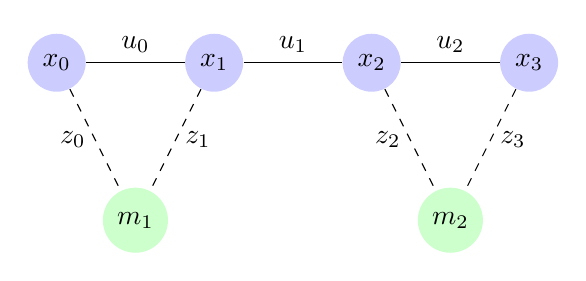
\begin{tikzpicture}
% Draw the nodes used for the picture
\node[circle,fill=blue!20](a){$x_0$};
\node[circle,fill=blue!20,right of=a,node distance=2cm](b){$x_1$};
\node[circle,fill=blue!20,right of=b,node distance=2cm](c){$x_2$};
\node[circle,fill=blue!20,right of=c,node distance=2cm](d){$x_3$};
\node(e) at ($(a)!0.5!(b)$){};
\node(f) at ($(c)!0.5!(d)$){};
\node[circle,fill=green!20,below of=e,node distance=2cm](g){$m_1$};
\node[circle,fill=green!20,below of=f,node distance=2cm](h){$m_2$};

% Draw the edges between the nodes
\draw (a) -- node[above]{$u_0$} (b);
\draw (b) -- node[above]{$u_1$} (c);
\draw (c) -- node[above]{$u_2$} (d);
\draw[dashed] (a) -- node[left]{$z_0$} (g);
\draw[dashed] (b) -- node[right]{$z_1$} (g);
\draw[dashed] (c) -- node[left]{$z_2$} (h);
\draw[dashed] (d) -- node[right]{$z_3$} (h);
\end{tikzpicture}
\caption{text}
\end{figure}

The edges form a set of \textit{information constraints}. To compute a map posterior, GraphSLAM linearises the set of constraints which results in a sparse information matrix and an information vector. 

\subsubsection{GraphSlam Back End}

\subsubsection{RTAB Map Impementation}


\section{Scene and robot configuration}
\subsection{Robot Model}
A robot model with simple geometries was selected for use in the SLAM simulation. The chassis is a rectangular prisim, and two wheels are located either side of the chassis centre forming a differential drive configuration - the robot model can be seein in Figure XXXX. An RGBD camera, front mounted on the chassis, provides 3D point cloud data of the environment and is represented by a red cube. Finally, a laser range finder is mounted on top of the robot providing 2D planar depth information.\\

\begin{figure}[h]
\begin{minipage}{0.45\textwidth}
	\centering
	\frame{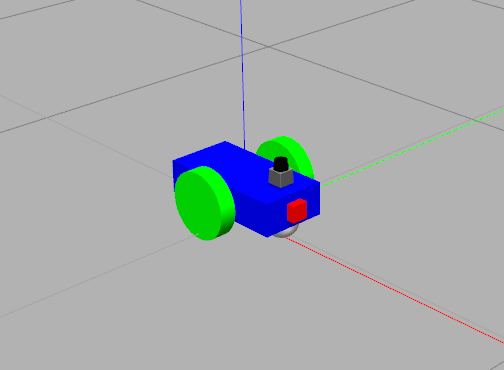
\includegraphics[scale=0.35]{robot_model}}
	\caption{text}
\end{minipage}
\hspace{1cm}
\begin{minipage}{0.45\textwidth}
	\captionof{table}{heading}
	\begin{tabular}{ll}
		\toprule
		\textbf{Link} & \textbf{Parent Link} \\
		\midrule
		\texttt{robot\_footprint} & \texttt{odom} \\
		\texttt{chassis} & \texttt{robot\_footprint} \\
		\texttt{camera} & \texttt{chassis} \\
		\texttt{hokuyo} & \texttt{chassis} \\
		\texttt{left\_wheel} & \texttt{chassis} \\
		\texttt{right\_wheel} & \texttt{chassis} \\
		\texttt{camera\_link\_optical} & \texttt{camera} \\
		\bottomrule
	\end{tabular}
\end{minipage}
\end{figure}

A full list of the links used to construct the robot model in the \texttt{graph\_slam\_bot.xacro} xml file can be seen in Table XXXX. Pictorially, the 3D coordinate frame hierachy is shown in Figure XXXX. This shows the coordinate frame attached to each link, in addition to the coordinate fram used for odometry. Note that arrows go from parent frames to child frames.

\clearpage

\begin{sidewaysfigure}[h]
	\centering
	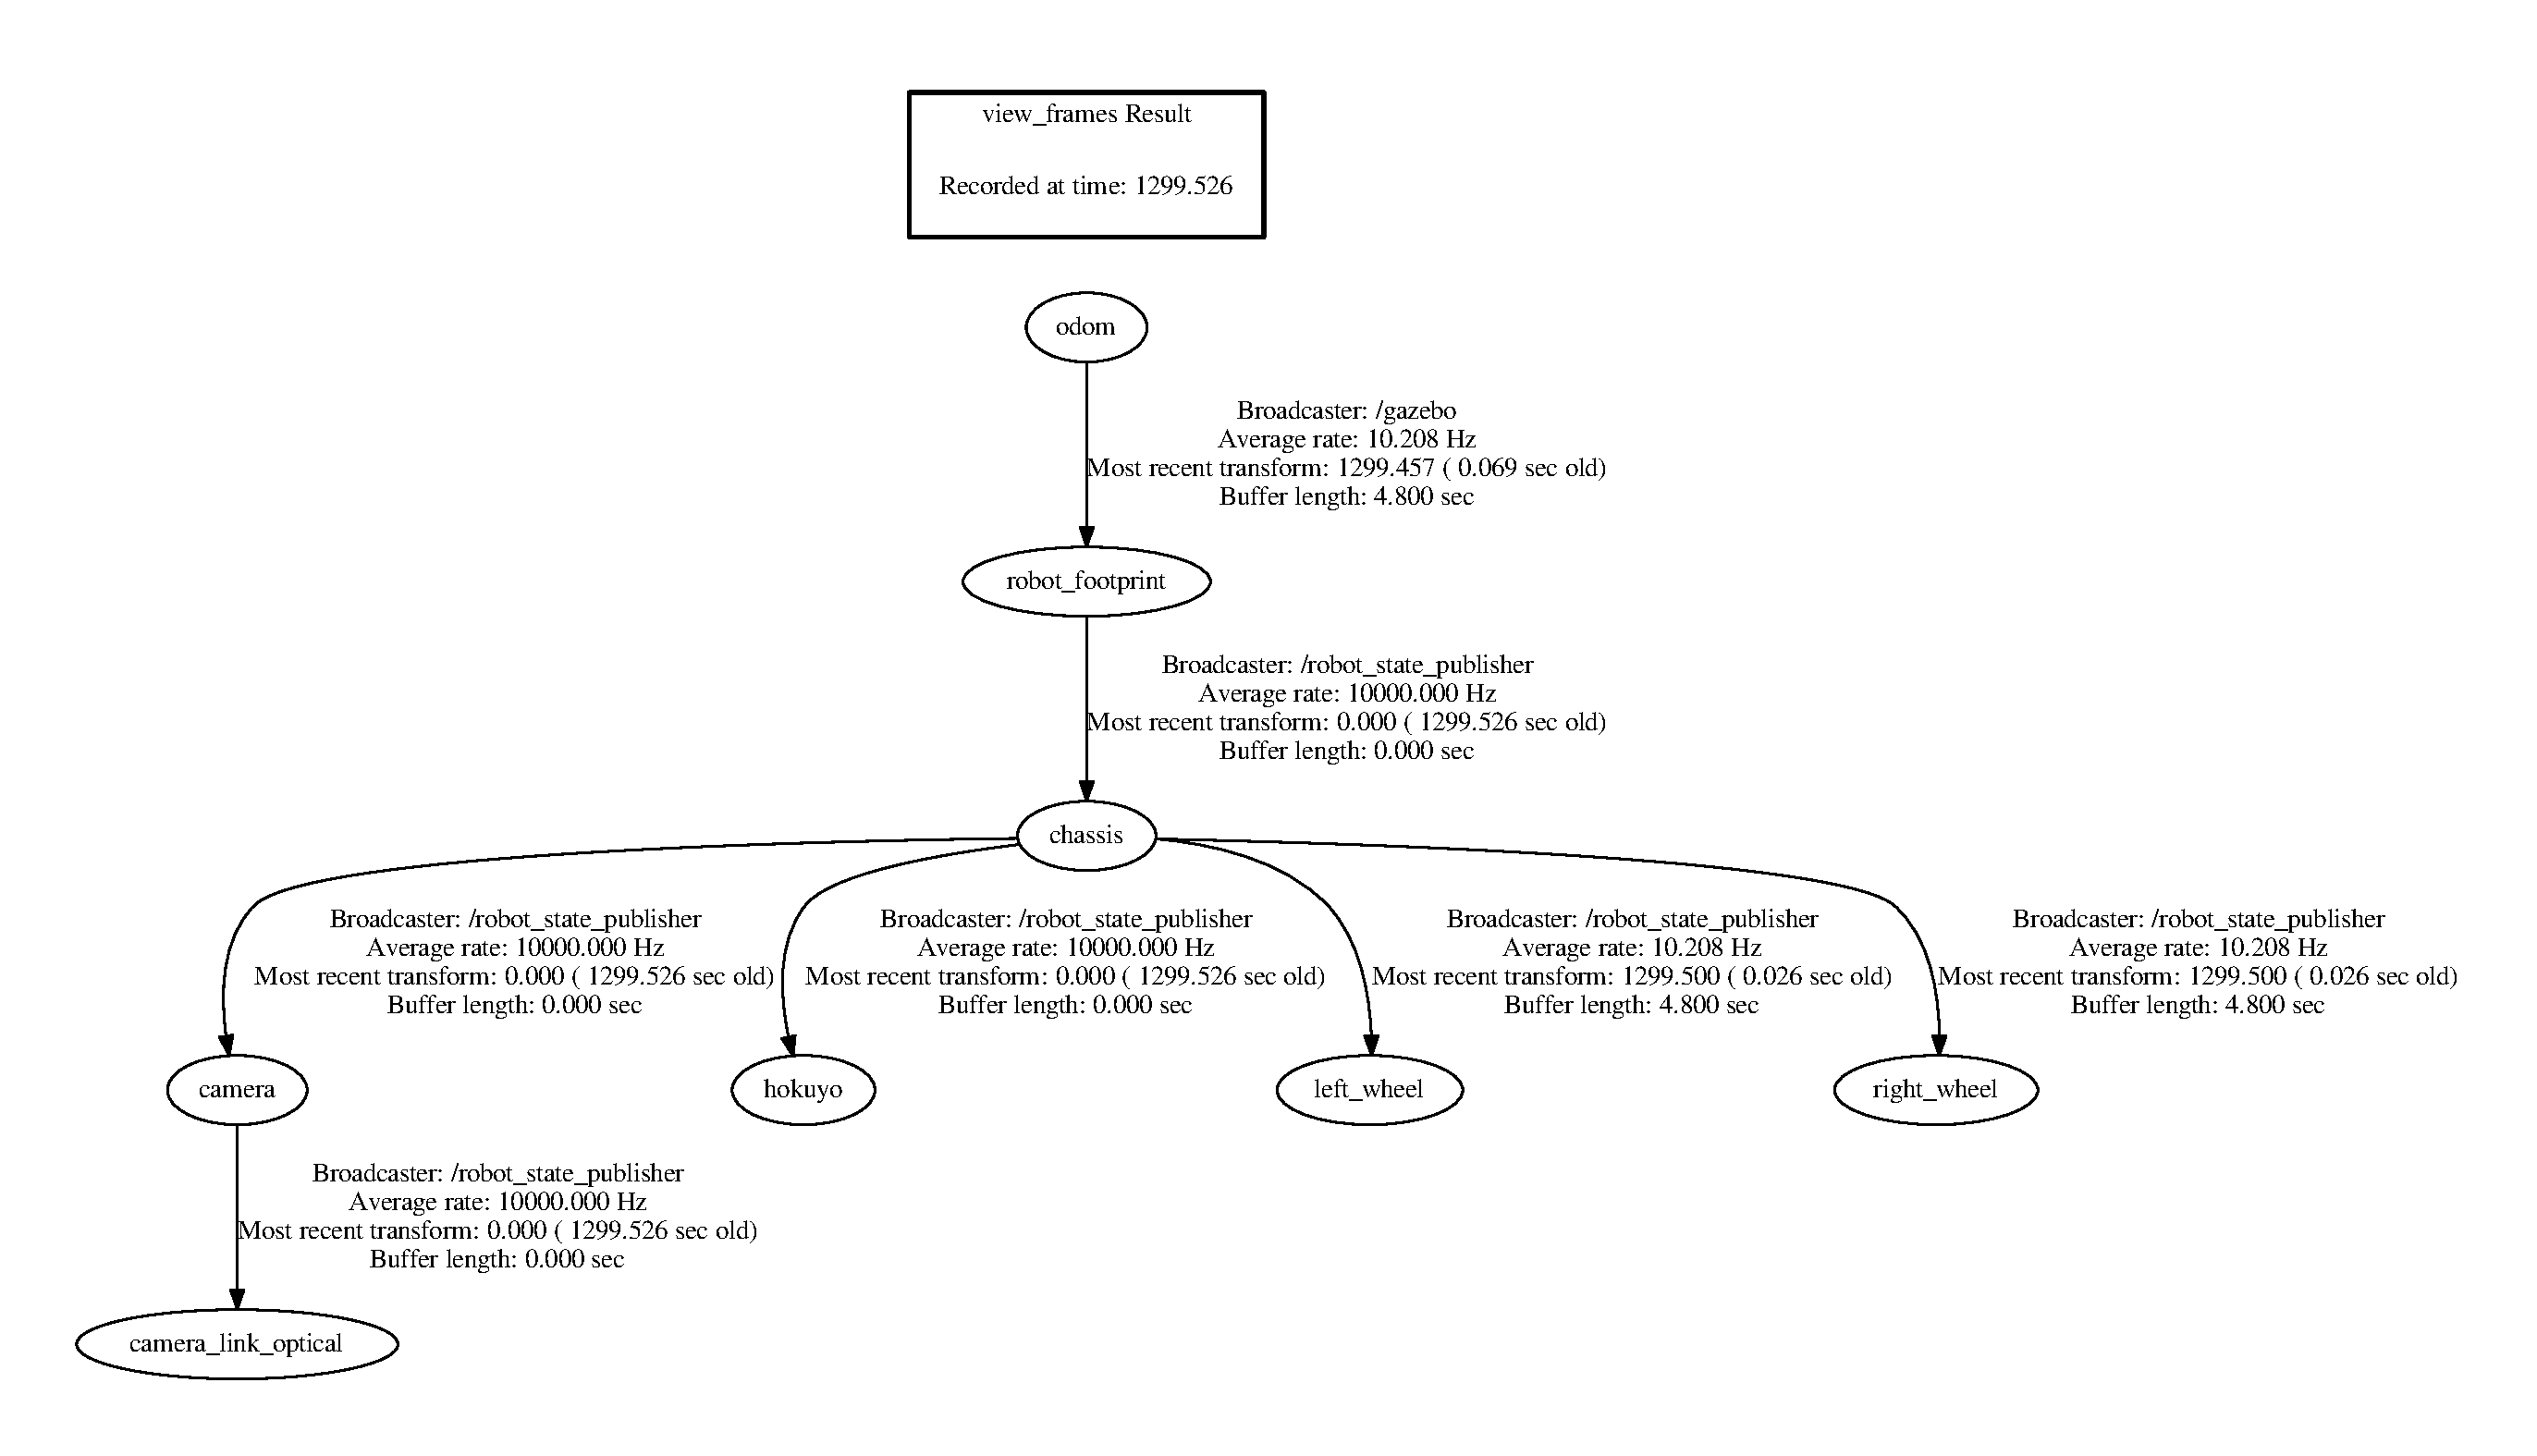
\includegraphics[scale=0.5]{frames}
	\caption{text}
\end{sidewaysfigure}

\clearpage

RTAB-Map is the package used to equip the robot model with GraphSLAM capabilities. The package uses RGB-D or stereo cameras and Lidar, meaning that there is some configuration of the RTAB-Map node to ensure that it is correctly subscribed to the correct topics published from the robot model sensors. A block diagram of the suggested configuration for robot models employing both RGB-D and Lidar can be seen in Figure XXXX. Notably, there are three topics for subsctiption from the RGB-D camera: RGB Image, Camera Info, and Image Depth. The Laser Scan and Odometry need to be subscribed from the published Lidar and rotary encoders topics, respectively.

\begin{figure}[h]
	\centering
	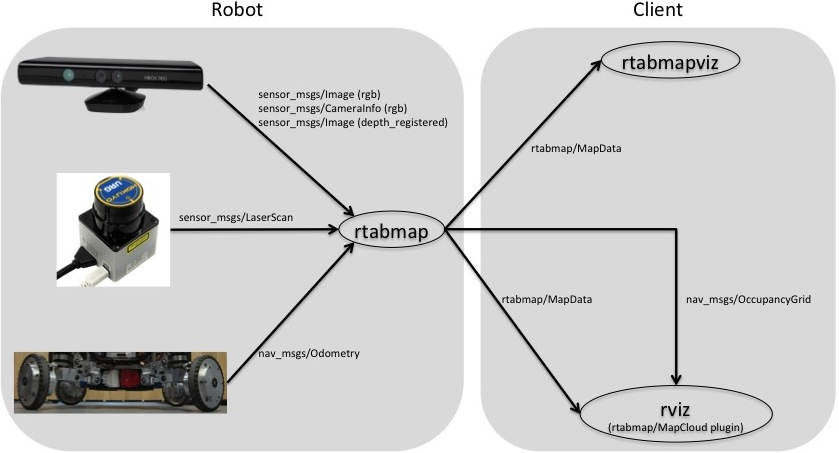
\includegraphics[scale=0.5]{rtabmap_setup}
	\caption{text}
\end{figure}

\begin{table}[h]
	\centering
	\caption{text}
	\begin{tabular}{ll}
		\toprule
		\textbf{Sensor Topic} & \textbf{Topic Path} \\
		\midrule
		RGBD Camera Image & \texttt{/camera\_ir/rgb/image\_raw} \\
		RGBD Camera Depth & \texttt{/camera\_ir/depth/image\_raw} \\
		RGBD Camera Info & \texttt{/camera\_ir/rgb/camera\_info} \\
		Laser Scan & \texttt{/graph\_slam\_bot/laser/scan} \\
		Odometry & \texttt{} \\ 
		\bottomrule
	\end{tabular}
\end{table}

\begin{figure}[h]
	\begin{minipage}{0.45\textwidth}
		text
	\end{minipage}
	\hspace{0.5cm}
	\begin{minipage}{0.45\textwidth}
		\centering
		\captionof{table}{text}
		\begin{tabular}{cc}
			\toprule
			\textbf{Parameter} & \textbf{Value}\\
			\midrule
			\texttt{Grid/FromDepth} & \texttt{false} \\
			\texttt{subscribe\_scan} & \texttt{true} \\
			\texttt{subscribe\_depth} & \texttt{true} \\
			\bottomrule
		\end{tabular}
	\end{minipage}
\end{figure}

\clearpage

\begin{sidewaysfigure}[h]
	\centering
	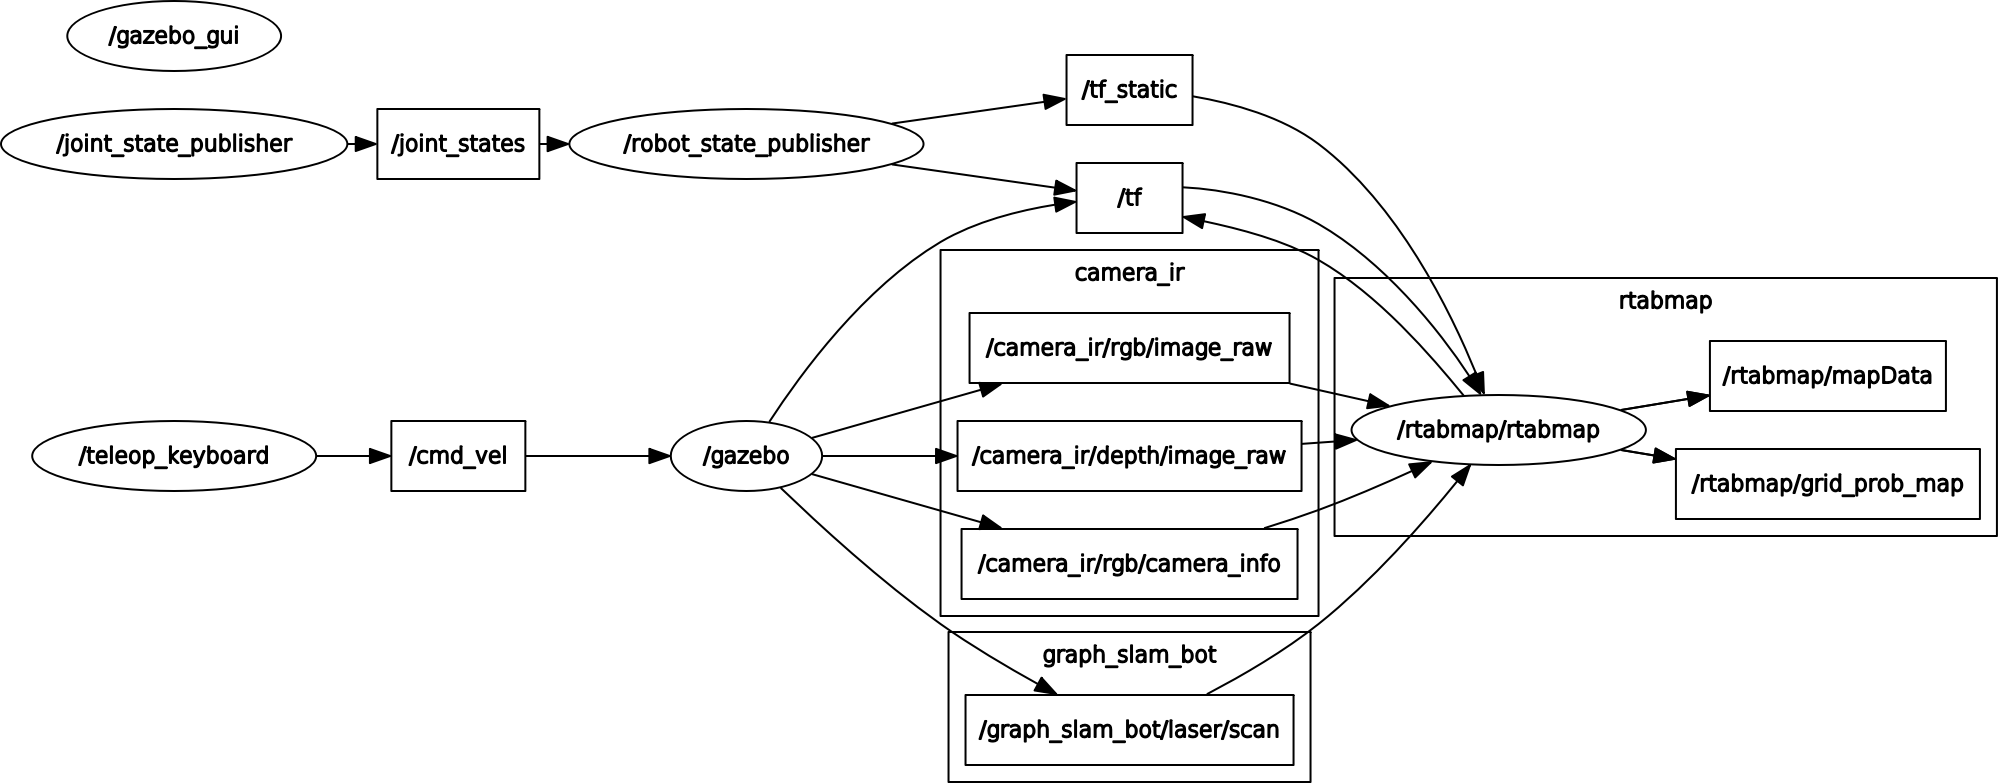
\includegraphics[scale=0.4]{rosgraph}
	\caption{text}
\end{sidewaysfigure}

\clearpage


WHAT ARE THE MAIN FILES THAT WERE REQUIRED TO CONFIGURE THE ROBOT

TALK ABOUT THE LAUNCH FILES THAT WERE CREATED TO LAUNCH EACH OF THE RESPECTIVE NODES


\subsection{Environment Model}
Rtab-Map was tested in two different environment models: a benchmark model, and an alternative model. Models have differing topologies, sizes, and features. 

\subsubsection{Benchmark Environment}
The benchmark model is of a small apartment mock up, featuring a kitchen and lounge room. The model is highly textured and contains many features - a good representation of real world environments. Rtab-Map should perform well in this environment because it is visually rich providing many opportunities for loop closure. The robot spawn point is in the kitchen. The benchmark environment model can be seen in Figure XXXX.
\begin{figure}[h]
\centering
\frame{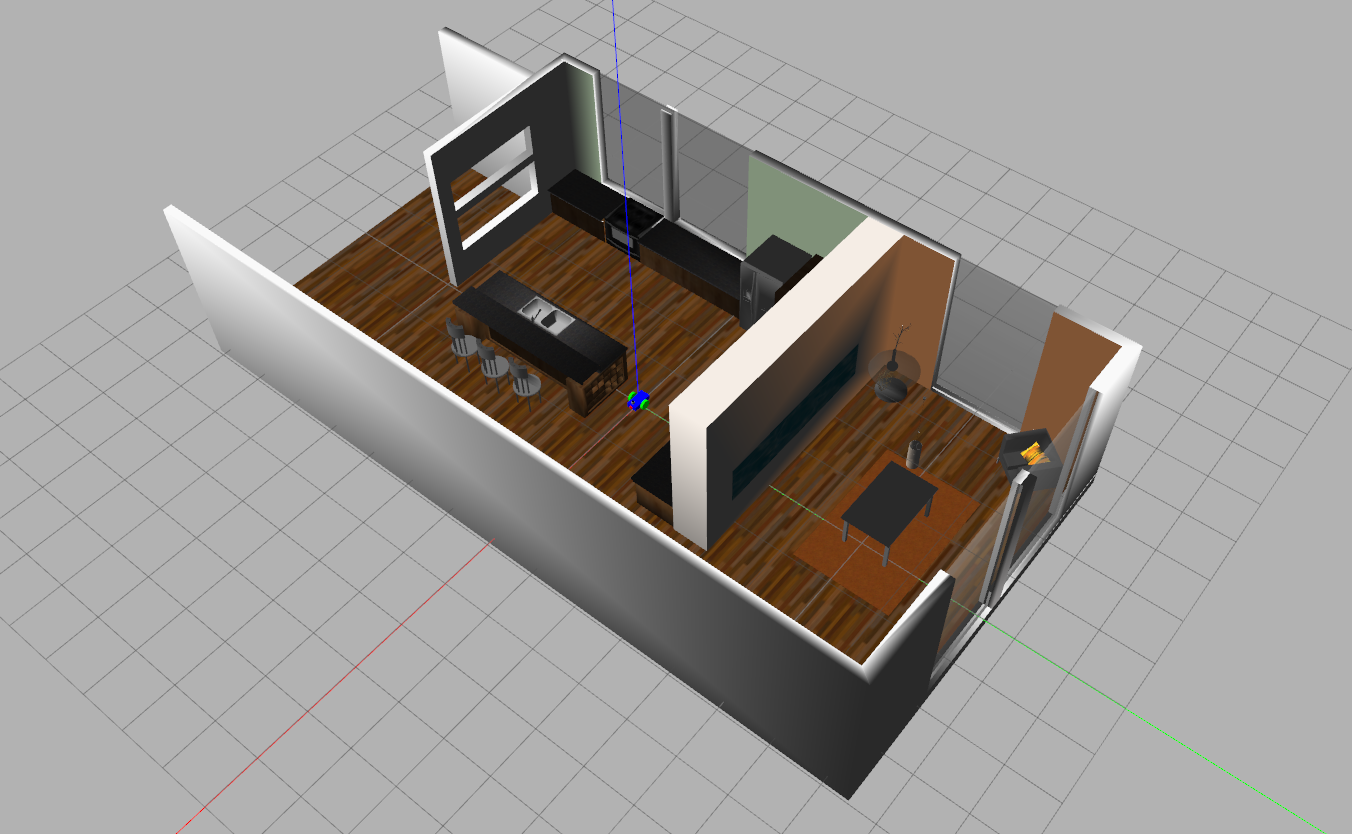
\includegraphics[scale=0.3]{benchmark_env}}
\caption{text}
\end{figure}

\subsubsection{Alternative Environment}
The alternative model was designed to be very simple. The topology is a basic rectangular room. An important design feature is the variation of features in the environment: some areas have many features, and other areas are featureless. This design choice was made to help evaluate Rtab-Map's performance in sections of the environment that are visually bland, or that have repetitive textures. The environment model was developed using the building editor embedded in Gazebo. The alternative environment model can be seen in Figure XXXX.
\begin{figure}
\centering
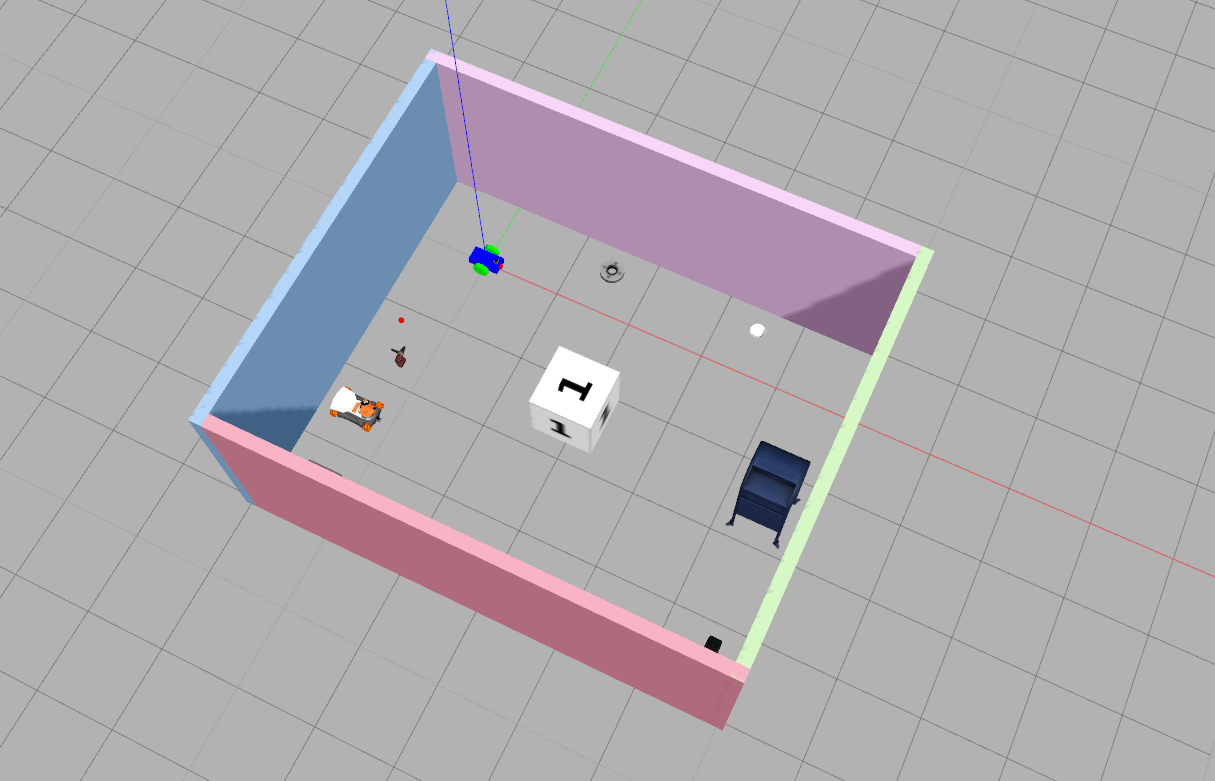
\includegraphics[scale=0.3]{alternative_env}
\caption{text}
\end{figure}


\section{Results}
\subsection{Benchmark Environment}
A teleop node was set up to manoeuvre the robot around the benchmark environment using keyboard input control. Approximately three laps of the kitchen, balcony, and lounge room areas were performed. Figure XXXX shows a final iteration of the 2D occupancy grid map, in addition to blue line which represents the robot's node graph through the environment, which is optimised by GraphSLAM in Rtab-Map. The red lines connecting nodes show loop closure activity. The red and green coordinate axes show the robot's starting location.
\begin{figure}[h]
\centering
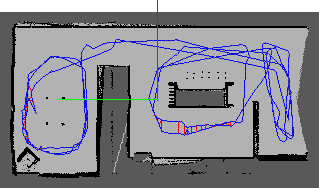
\includegraphics[scale=0.8]{kitchen_graph_view}
\caption{text}
\end{figure}

As the robot traverses the environment Rtab-Map identifies features from images using the \texttt{SURF} detection algorithm which was specified in the mapping node configuration. Figure XXXX shows a single image along the robot path, taken from the Rtab-Map database. The yellow highlights identify features that \texttt{SURF} has identified. As images are collected along the robot path, features in new images are compared to features from old images. The pink highlights represent instances where two images have features in common. These common features are used to create neighbouring links between images and loop closures. Figure XXXX shows the constraint view for the same point in time as Figure XXXX - this shows where the neighbouring links and loop closures were created.
\begin{figure}[h]
\centering
\begin{minipage}[t]{0.45\textwidth}
\centering
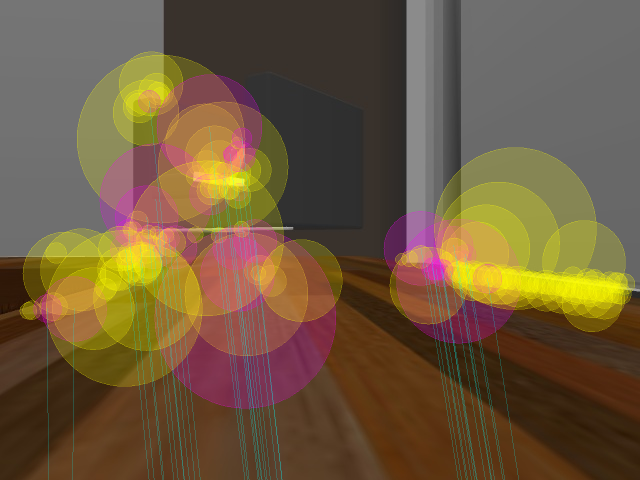
\includegraphics[height=5.5cm]{kitchen_features}
\caption{text}
\end{minipage}
\hspace{1cm}
\begin{minipage}[t]{0.45\textwidth}
\centering
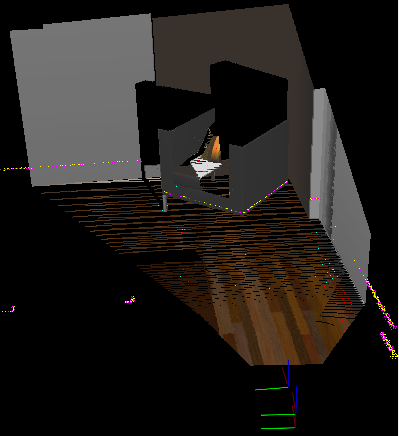
\includegraphics[height=5.5cm]{kitchen_constraints}
\caption{text}
\end{minipage}
\end{figure}

NEED TO TALK MORE ABOUT THE DIFFERENT LOOP CLOSURE ACTIVITY AND ACTIVITY WHERE THERE WAS NO LOOP CLOSURE.

Rtab-Map successfully created a 3D map from captured point cloud data captured by the RGBD camera. The 3D environment model was of reasonable fidelity, and well aligned with the 2D occupancy grid. Figure XXXX shows the 3D environment model from Rviz.
\begin{figure}[h]
\centering
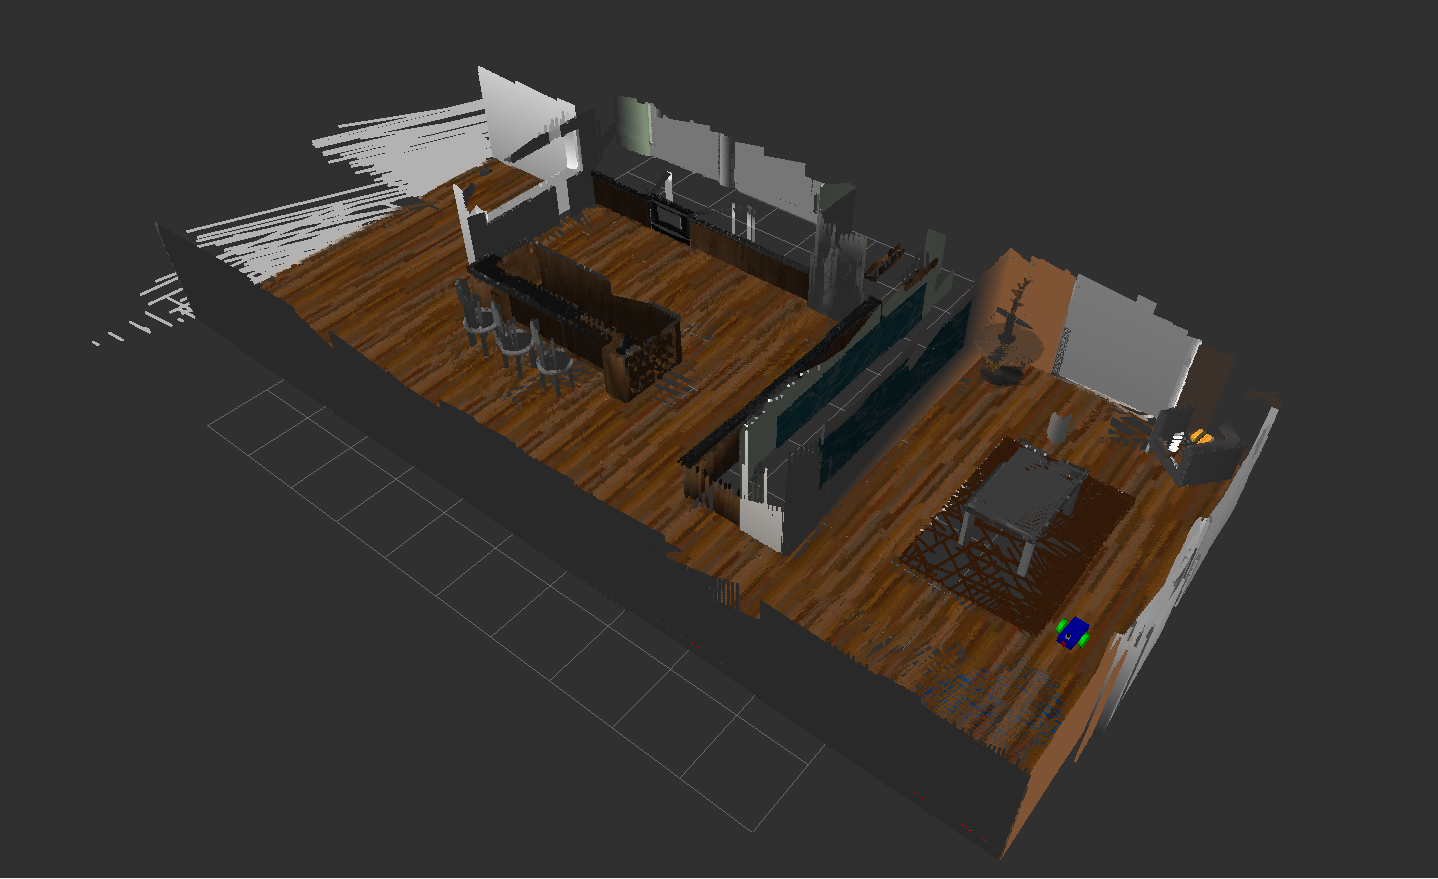
\includegraphics[scale=0.28]{kitchen_3d_map_2}
\caption{text}
\end{figure}

The robot was able to successfully localise within the mapped environment, making small corrections to the odometry upon detection of loop closure.


\subsection{Alternative Environment}
As with the benchmark model, the robot was manoeuvred through the alternative environment using keyboard commands issued to a teleop node. Three laps of the basic environment were undertaken. The final iteration of the 2D occupancy grid map can be seen in Figure XXXX. The node graph used by GraphSLAM in Rtab-Map is represented by the blue line, and loop closure activity is shown in red.
\begin{figure}[h]
\centering
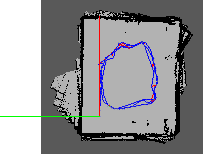
\includegraphics[scale=1.2]{slam_house_2_graph_view}
\caption{text}
\end{figure}

\begin{figure}[h]
\centering
\begin{minipage}{0.45\textwidth}
\centering
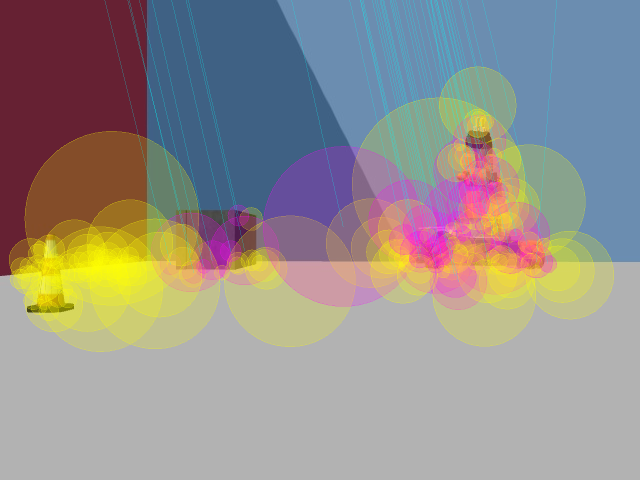
\includegraphics[height=5.5cm]{slam_house_features_corner_1}
\caption{text}
\end{minipage}
\hspace{1cm}
\begin{minipage}{0.45\textwidth}
\centering
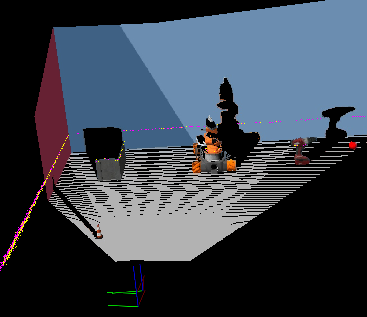
\includegraphics[height=5.5cm]{slam_house_constraints_1}
\caption{text}
\end{minipage}
\end{figure}

\begin{figure}[h]
\centering
\begin{minipage}{0.45\textwidth}
\centering
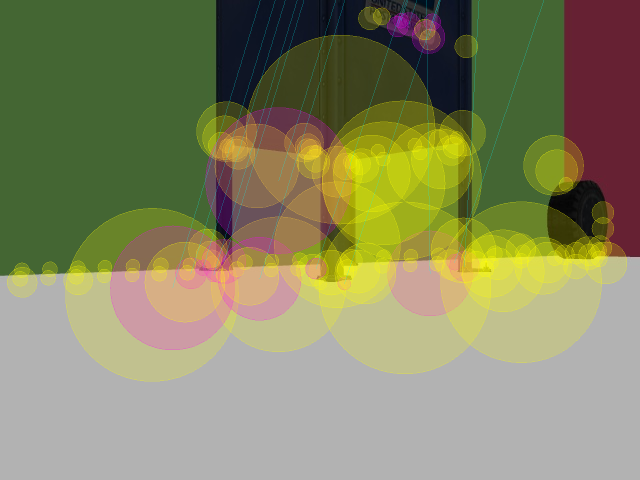
\includegraphics[height=5.5cm]{slam_house_features_corner_2}
\caption{text}
\end{minipage}
\hspace{1cm}
\begin{minipage}{0.45\textwidth}
\centering
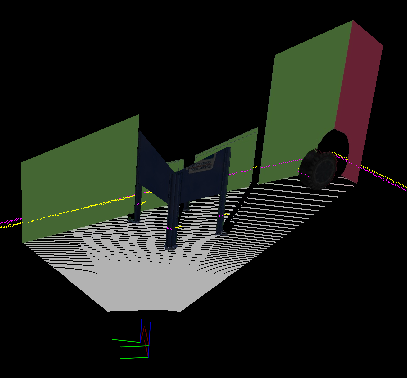
\includegraphics[height=5.5cm]{slam_house_constraints_2}
\caption{text}
\end{minipage}
\end{figure}

\begin{figure}[h]
\centering
\begin{minipage}{0.45\textwidth}
\centering

\includegraphics[height=5.5cm]{slam_house_features_corner_3}
\caption{text}
\end{minipage}
\hspace{1cm}
\begin{minipage}{0.45\textwidth}
\centering
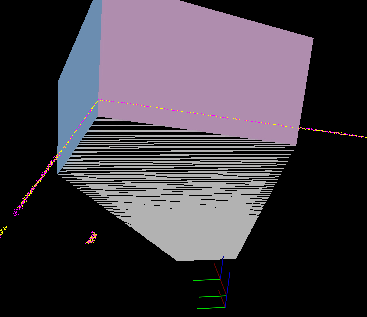
\includegraphics[height=5.5cm]{slam_house_constraints_3}
\caption{text}
\end{minipage}
\end{figure}


\section{Discussion}
Discussion - The student explains how the procedure went and methodologies to improve it. The student should compare and contrast the performance of RTAB Mapping in different worlds.


\section{Future Work}


\bibliography{my_bib}
\bibliographystyle{ieeetr}

\end{document}